\section{Boot and software}
\label{sec:boot}

\subsection{Reset}

The top level (\src{rtl/doomacracy.vhd}) has three reset sources:

\begin{itemize}
  \item Power-on. An 8-bit counter holds \texttt{reset} high for 256 cycles after FPGA configuration.
  \item KEY0. The key goes through two flip-flops. \texttt{reset} is high while the key is pushed.
  \item The syscon reboot command. It restarts the power-on counter.
\end{itemize}

The CPU, the caches and the bus use a second signal, \texttt{cpu\_reset}. This signal stays high until the SDRAM controller completes its initialization. Figure~\ref{fig:resetseq} shows the sequence after power-on.

\begin{figure}[H]
  \centering
  \begin{tikzpicture}[font=\scriptsize]
    \node[box, text width=2.6cm, minimum height=0.9cm] (a) at (0,0) {power-on counter\\256 cycles};
    \node[box, text width=3.0cm, minimum height=0.9cm] (b) at (3.8,0) {SDRAM initialization\\approx. 10,100 cycles};
    \node[box, text width=2.6cm, minimum height=0.9cm] (c) at (7.6,0) {caches clear tags\\512 cycles};
    \node[box, text width=2.6cm, minimum height=0.9cm] (d) at (11.2,0) {CPU fetches\\address \texttt{0x0}};
    \draw[tr] (a) -- (b);
    \draw[tr] (b) -- (c);
    \draw[tr] (c) -- (d);
    \draw[decorate, decoration={brace, mirror, amplitude=4pt}] (a.south west) ++(0,-0.15) -- ($(a.south east)+(0,-0.15)$) node[midway, below=6pt] {\texttt{reset} = 1};
    \draw[decorate, decoration={brace, mirror, amplitude=4pt}] (a.south west) ++(0,-1.0) -- ($(b.south east)+(0,-1.0)$) node[midway, below=6pt] {\texttt{cpu\_reset} = 1};
  \end{tikzpicture}
  \caption{The sequence after power-on}
  \label{fig:resetseq}
\end{figure}

\subsection{Boot ROM}

The boot ROM is 4 KB at address 0. Its source is \src{sw/boot/boot.c}. The build converts the binary to a VHDL constant (\src{rtl/boot_rom_data.vhd}). The boot ROM does these tasks:

\begin{itemize}
  \item If SW9 is up, it receives a flash image through JTAG.
  \item It reads the header of the flash image and identifies a Doom image or a Linux image.
  \item It copies the image to RAM and jumps to it.
\end{itemize}

Figure~\ref{fig:bootflow} shows the main sequence. The value on the HEX display shows the current step.

\begin{figure}[H]
  \centering
  \begin{tikzpicture}[font=\scriptsize]
    \node[box, text width=4.2cm] (s0) at (0,0) {start: HEX = \texttt{B001}};
    \node[decision] (d1) at (0,-1.6) {SW9 up?};
    \node[box, text width=3.6cm] (j) at (6.2,-1.6) {JTAG load\\(Figure~\ref{fig:jtagflow})};
    \node[box, text width=4.2cm] (s1) at (0,-3.2) {read the magic word at flash address 0};
    \node[decision] (d2) at (0,-4.8) {``LNUX''?};
    \node[box, text width=3.6cm] (lx) at (6.2,-4.8) {Linux boot\\HEX = \texttt{B104}, \texttt{B105}};
    \node[decision] (d3) at (0,-6.4) {``DOOM''?};
    \node[box, text width=3.6cm] (e1) at (6.2,-6.4) {error \texttt{E001}};
    \node[box, text width=4.2cm] (s2) at (0,-8.0) {check the load address, the length\\and the entry address};
    \node[box, text width=4.2cm] (s3) at (0,-9.5) {HEX = \texttt{B002}: copy the firmware\\from flash \texttt{0x100} to the load address};
    \node[box, text width=4.2cm] (s4) at (0,-11.0) {HEX = \texttt{B003}: jump to the entry address};
    \draw[tr] (s0) -- (d1);
    \draw[tr] (d1) -- (j) node[cond, midway, above] {yes};
    \draw[tr] (d1) -- (s1) node[cond, midway, left] {no};
    \draw[tr] (j.south) |- (s1.east);
    \node[cond, right] at (6.2,-2.6) {image is in flash};
    \draw[tr] (s1) -- (d2);
    \draw[tr] (d2) -- (lx) node[cond, midway, above] {yes};
    \draw[tr] (d2) -- (d3) node[cond, midway, left] {no};
    \draw[tr] (d3) -- (e1) node[cond, midway, above] {no};
    \draw[tr] (d3) -- (s2) node[cond, midway, left] {yes};
    \draw[tr] (s2) -- (s3);
    \draw[tr] (s3) -- (s4);
  \end{tikzpicture}
  \caption{The boot ROM sequence}
  \label{fig:bootflow}
\end{figure}

\subsubsection{JTAG load}
The host script \src{tools/jtag_flash.tcl} sends the image (Figure~\ref{fig:jtagstream}). The boot ROM stores the image in the top 4 MB of SDRAM, at \texttt{0x2040\_0000}. The flash is much slower than JTAG, so the boot ROM receives the full image before it writes the flash. Figure~\ref{fig:jtagflow} shows the sequence.

\begin{figure}[H]
  \centering
  \begin{tikzpicture}[font=\scriptsize]
    \node[box, text width=6.4cm] (a) at (0,0) {HEX = \texttt{1000}: wait for the magic word,\\then read the word count $n$};
    \node[box, text width=6.4cm] (b) at (0,-1.6) {HEX = \texttt{1xxx}: receive $n$ words into SDRAM\\and add them};
    \node[box, text width=6.4cm] (c) at (0,-3.2) {compare the sum with the checksum, then read\\the image from SDRAM and compare again};
    \node[decision] (d) at (0,-4.9) {SW8 up?};
    \node[box, text width=3.4cm] (lx) at (6.8,-4.9) {Linux boot from the\\SDRAM buffer};
    \node[box, text width=6.4cm] (e) at (0,-6.6) {compare the next 64 KB region of the image\\with the flash};
    \node[decision] (f) at (0,-8.3) {different?};
    \node[box, text width=3.4cm] (g) at (6.8,-8.3) {HEX = \texttt{20rr}: erase\\HEX = \texttt{30rr}: program\\then verify};
    \node[decision] (k) at (0,-10.3) {last region?};
    \node[box, text width=6.4cm] (h) at (0,-12.0) {HEX = \texttt{600D}: continue with the boot ROM sequence};
    \draw[tr] (a) -- (b);
    \draw[tr] (b) -- (c);
    \draw[tr] (c) -- (d);
    \draw[tr] (d) -- (lx) node[cond, midway, above] {yes};
    \draw[tr] (d) -- (e) node[cond, midway, left] {no};
    \draw[tr] (e) -- (f);
    \draw[tr] (f) -- (g) node[cond, midway, above] {yes};
    \draw[tr] (f) -- (k) node[cond, midway, left] {no};
    \draw[tr] (g.south) |- (k.east);
    \draw[tr] (k.west) -- (-4.6,-10.3) |- (e.west);
    \node[cond, above] at (-3.4,-10.3) {no};
    \draw[tr] (k) -- (h) node[cond, midway, left] {yes};
  \end{tikzpicture}
  \caption{The JTAG load sequence. \texttt{rr} is the region number.}
  \label{fig:jtagflow}
\end{figure}

The boot ROM writes only the regions that are different. If the flash already holds the image, the boot ROM writes nothing. For each region that is different, the boot ROM does these steps:

\begin{enumerate}
  \item For each 8 KB block that is not blank, send the sector erase command. Then read status bit DQ7 until the erase completes.
  \item For each byte that is not \texttt{FF}, send the byte program command. Then read DQ7 until the program completes.
  \item Compare the region with the image.
\end{enumerate}

If SW8 and SW9 are up, the image must be a Linux image. The boot ROM starts Linux from the SDRAM buffer and does not change the flash.

\subsubsection{Display codes}
Table~\ref{tab:hexcodes} lists the values on the HEX display.

\begin{guidetable}{HEX display codes}{hexcodes}{l l}
HEX & meaning \\
\midrule
\texttt{B001} & The boot ROM has started. \\
\texttt{1xxx} & JTAG receive. \texttt{xxx} is the number of words received, divided by 1024. \\
\texttt{20rr} & Erase of flash region \texttt{rr}. \\
\texttt{30rr} & Program of flash region \texttt{rr}. \\
\texttt{600D} & The JTAG load is complete. LEDR shows the number of regions written. \\
\texttt{B002} & Copy of the Doom firmware from flash to SRAM. \\
\texttt{B003} & Jump to the Doom firmware. \\
\texttt{B104} & Copy of the Linux kernel and the device tree to SDRAM. \\
\texttt{B105} & Jump to the Linux kernel. \\
\texttt{D000} & Doom has started its platform code. \\
\texttt{00FF} & Power off (syscon). \\
\texttt{Ennn} & Error \texttt{nnn}. See Table~\ref{tab:errcodes}. \\
\end{guidetable}

When an error occurs, the boot ROM stops. All red LEDs come on, and the UART sends the error code and a value. The HEX display shows three values in sequence, one each second: the code \texttt{Ennn}, the high half of the value, the low half of the value.

\begin{guidetable}{Boot ROM error codes}{errcodes}{l l l}
code & cause & value \\
\midrule
\texttt{E001} & The magic word is not ``DOOM'' or ``LNUX''. & the magic word \\
\texttt{E002} & The load address or the length is not correct. & the length \\
\texttt{E003} & The entry address is not in the firmware. & the entry address \\
\texttt{E004} & The firmware returned to the boot ROM. & the entry address \\
\texttt{E005} & The kernel or the device tree is too large. & the kernel length \\
\texttt{E010} & The JTAG image is larger than 4 MB. & the word count \\
\texttt{E011} & The JTAG checksum is not correct. & the calculated sum \\
\texttt{E012} & The JTAG FIFO had an overflow. & the word count \\
\texttt{E013} & A flash erase did not complete. & flash status \\
\texttt{E014} & A flash byte program did not complete. & flash status \\
\texttt{E015} & The flash data is different from the image. & the flash address \\
\texttt{E016} & SW8 is up and the image is not a Linux image. & the magic word \\
\texttt{E017} & The image in SDRAM changed after the receive. & the second sum \\
\end{guidetable}

\subsection{Flash image}

The script \src{tools/mkflash.py} builds the Doom flash image (Figure~\ref{fig:flashimg}). The header is six 32-bit little-endian words (Table~\ref{tab:flashhdr}).

\begin{figure}[H]
  \centering
  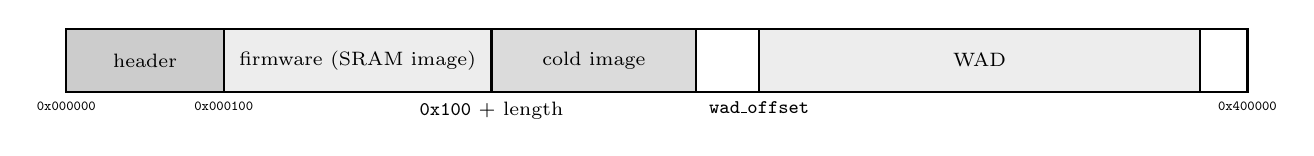
\begin{tikzpicture}[font=\scriptsize]
    \draw[thick, fill=black!20] (-0.8,0) rectangle (1.2,0.8);  \node at (0.2,0.4) {header};
    \draw[thick, fill=black!7]  (1.2,0) rectangle (4.6,0.8); \node at (2.9,0.4) {firmware (SRAM image)};
    \draw[thick, fill=black!14] (4.6,0) rectangle (7.2,0.8); \node at (5.9,0.4) {cold image};
    \draw[thick, fill=white]    (7.2,0) rectangle (8.0,0.8);
    \draw[thick, fill=black!7]  (8.0,0) rectangle (13.6,0.8); \node at (10.8,0.4) {WAD};
    \draw[thick, fill=white]    (13.6,0) rectangle (14.2,0.8);
    \node[below, font=\ttfamily\tiny] at (-0.8,0) {0x000000};
    \node[below, font=\ttfamily\tiny] at (1.2,0) {0x000100};
    \node[below, align=center] at (4.6,0) {\texttt{0x100} + length};
    \node[below, align=center] at (8.0,0) {\texttt{wad\_offset}};
    \node[below, font=\ttfamily\tiny] at (14.2,0) {0x400000};
  \end{tikzpicture}
  \caption{The Doom flash image (not to scale)}
  \label{fig:flashimg}
\end{figure}

\begin{guidetable}{Flash header}{flashhdr}{l l l}
offset & field & contents \\
\midrule
\texttt{+0x00} & magic & \texttt{0x4D4F4F44} (``DOOM'') \\
\texttt{+0x04} & load\_addr & \texttt{0x1000\_0000}. The boot ROM copies the firmware to this address. \\
\texttt{+0x08} & length & Firmware length in bytes, a multiple of 4. \\
\texttt{+0x0C} & entry & The boot ROM jumps to this address. \\
\texttt{+0x10} & wad\_offset & Offset of the WAD in flash, a multiple of 4 KB. \\
\texttt{+0x14} & wad\_length & WAD length in bytes. \\
\end{guidetable}

The WAD is the shareware \texttt{doom1.wad}. The script \src{tools/wad_strip.py} sets the length of each sound, music and ENDOOM lump to zero. The WAD directory does not change. The result is approximately 3.41 MB, which fits in the 4 MB flash with the firmware.

\subsubsection{Linux image}
A Linux image has the magic word \texttt{0x58554E4C} (``LNUX''). The header holds the kernel length (\texttt{+4}), the device tree offset (\texttt{+8}) and the device tree length (\texttt{+12}). The kernel starts at \texttt{0x100}. The boot ROM does these steps:

\begin{enumerate}
  \item Copy the kernel to the start of SDRAM.
  \item Copy the device tree to the top 16 KB of SDRAM.
  \item Set \texttt{FB\_BASE} to \texttt{0x40000} and \texttt{VIDEO\_MODE} to 1 (RGB565), for the Linux console.
  \item Set register a0 to 0 and register a1 to the device tree address, \texttt{0x807F\_C000}.
  \item Jump to \texttt{0x8000\_0000}.
\end{enumerate}

\subsection{Doom firmware}

\subsubsection{Memory layout}
The linker script is \src{sw/doom/doom.ld}. The firmware is larger than the space in SRAM, so the linker script divides it into two images (Figure~\ref{fig:fwmem}):

\begin{itemize}
  \item The SRAM image holds the code and data that Doom uses in each frame.
  \item The cold image holds code that Doom uses only at startup, in menus and at a level load. It also holds most of the C library. The cold image runs from SDRAM.
\end{itemize}

\begin{figure}[H]
  \centering
  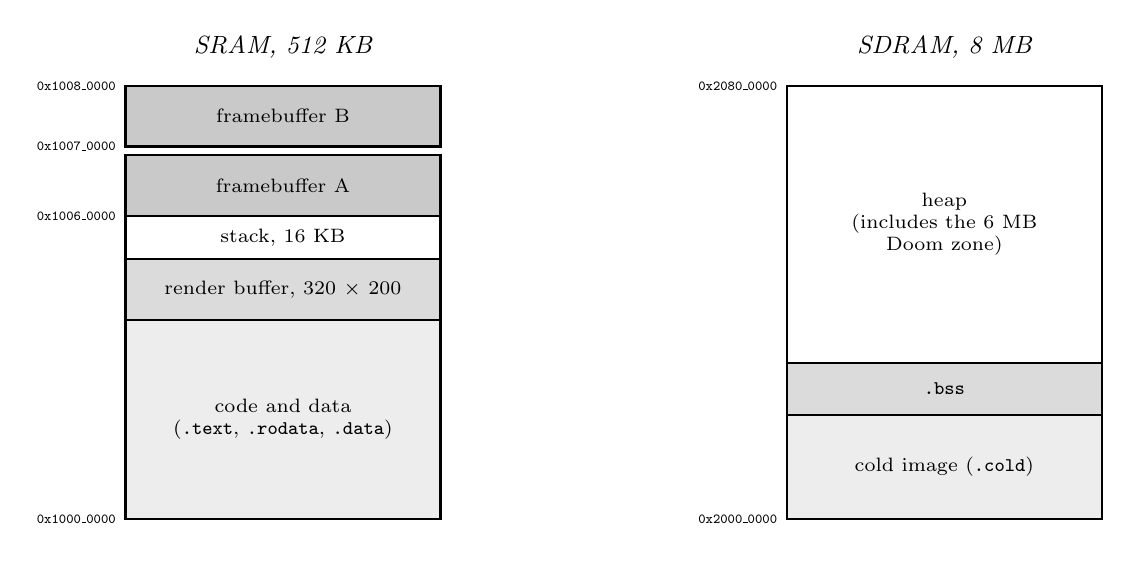
\begin{tikzpicture}[font=\scriptsize, y=0.55cm]
    \node[above, font=\small\itshape] at (2.0,10.4) {SRAM, 512 KB};
    \draw[thick, fill=black!7]  (0,0) rectangle (4.0,4.6);  \node[align=center] at (2.0,2.3) {code and data\\(\texttt{.text}, \texttt{.rodata}, \texttt{.data})};
    \draw[thick, fill=black!14] (0,4.6) rectangle (4.0,6.0); \node at (2.0,5.3) {render buffer, 320 $\times$ 200};
    \draw[thick, fill=white]    (0,6.0) rectangle (4.0,7.0); \node at (2.0,6.5) {stack, 16 KB};
    \draw[thick, fill=black!21] (0,7.0) rectangle (4.0,8.4); \node at (2.0,7.7) {framebuffer A};
    \draw[thick, fill=black!21] (0,8.6) rectangle (4.0,10.0); \node at (2.0,9.3) {framebuffer B};
    \node[left, font=\ttfamily\tiny] at (0,0) {0x1000\_0000};
    \node[left, font=\ttfamily\tiny] at (0,7.0) {0x1006\_0000};
    \node[left, font=\ttfamily\tiny] at (0,8.6) {0x1007\_0000};
    \node[left, font=\ttfamily\tiny] at (0,10.0) {0x1008\_0000};
    \begin{scope}[xshift=8.4cm]
      \node[above, font=\small\itshape] at (2.0,10.4) {SDRAM, 8 MB};
      \draw[thick, fill=black!7]  (0,0) rectangle (4.0,2.4);  \node[align=center] at (2.0,1.2) {cold image (\texttt{.cold})};
      \draw[thick, fill=black!14] (0,2.4) rectangle (4.0,3.6); \node at (2.0,3.0) {\texttt{.bss}};
      \draw[thick, fill=white]    (0,3.6) rectangle (4.0,10.0); \node[align=center] at (2.0,6.8) {heap\\(includes the 6 MB\\Doom zone)};
      \node[left, font=\ttfamily\tiny] at (0,0) {0x2000\_0000};
      \node[left, font=\ttfamily\tiny] at (0,10.0) {0x2080\_0000};
    \end{scope}
  \end{tikzpicture}
  \caption{Memory use of the Doom firmware (not to scale). Low addresses are at the bottom.}
  \label{fig:fwmem}
\end{figure}

\subsubsection{Startup}
The startup code is \src{sw/doom/crt0.S}. It does these steps:

\begin{enumerate}
  \item Set the global pointer and the stack pointer (\texttt{0x1006\_0000}).
  \item Copy the cold image from flash to SDRAM. The cold image is in flash immediately after the SRAM image.
  \item Set \texttt{.bss} to zero.
  \item Call the C library initialization and then \texttt{main}.
\end{enumerate}

\texttt{main} is in \src{sw/doom/doomgeneric_doomacracy.c}. It reads the game version from the first demo in the WAD and starts Doom. If SW0 is up, \texttt{main} adds the option \texttt{-timedemo demo1}.

\subsubsection{Video output}
Doom draws each frame into the render buffer in SRAM. The function \texttt{I\_FinishUpdate} (\src{sw/doom/i_video_doomacracy.c}) then moves the frame to the screen. There are two framebuffers, A and B. The video block shows one of them (the front buffer). Software writes the other (the back buffer).

\begin{enumerate}
  \item Wait until \texttt{FRAME\_COUNT} is different from the value at the last change of \texttt{FB\_BASE}. After this time, the video block does not read the back buffer.
  \item Copy the render buffer (64,000 bytes) to the back buffer.
  \item Write the address of the back buffer to \texttt{FB\_BASE}.
  \item Save \texttt{FRAME\_COUNT}. The two buffers change roles.
\end{enumerate}

Figure~\ref{fig:flip} shows the sequence. The video block uses the new \texttt{FB\_BASE} at the next vertical blanking.

\begin{figure}[H]
  \centering
  \begin{waveform}[1.45cm]{9}
    \wavebus{\texttt{FRAME\_COUNT}}{0/3/$n$, 3/6/$n+1$, 6/9/$n+2$}
    \wavebus{software}{0/2.25/draw, 2.25/3.75/copy to B, 3.75/6.25/draw, 6.25/7.75/copy to A, 7.75/9/draw}
    \wavebus{\texttt{FB\_BASE}}{0/3.75/A, 3.75/7.75/B, 7.75/9/A}
    \wavebus{on screen}{0/6/A, 6/9/B}
  \end{waveform}
  \caption{Double buffering. Each grid line is 1/3 of a VGA frame.}
  \label{fig:flip}
\end{figure}

\texttt{I\_SetPalette} writes the 256 palette entries to the \texttt{PALETTE} register.

\subsubsection{Keyboard}
\texttt{DG\_GetKey} reads all bytes from the \texttt{KBD} register and decodes them. PS/2 scan code set 2 uses two prefix bytes:

\begin{itemize}
  \item \texttt{F0}: the next byte is a key release.
  \item \texttt{E0}: the next byte is an extended key (for example, the arrow keys).
\end{itemize}

The decoder keeps one flag for each prefix. A key byte gives one key event, and then the decoder clears the flags. Table~\ref{tab:ps2ex} shows examples.

\begin{guidetable}{PS/2 byte sequences}{ps2ex}{l l l}
bytes & event & Doom key \\
\midrule
\texttt{1C} & A pushed & \texttt{a} \\
\texttt{F0 1C} & A released & \texttt{a} \\
\texttt{E0 74} & right arrow pushed & \texttt{KEY\_RIGHTARROW} \\
\texttt{E0 F0 74} & right arrow released & \texttt{KEY\_RIGHTARROW} \\
\texttt{14} & left Ctrl pushed & \texttt{KEY\_FIRE} \\
\texttt{29} & space pushed & \texttt{KEY\_USE} \\
\end{guidetable}

The hardware FIFO holds only 16 bytes. Thus \texttt{DG\_SleepMs} also reads the keyboard while it waits.

\subsubsection{Time and files}
\texttt{DG\_GetTicksMs} reads \texttt{TIMER\_US} and divides by 1000. The firmware extends the 32-bit register to 64 bits in software.

The only file is \texttt{doom1.wad}. A read of the file copies bytes from the WAD in flash. Standard output goes to the UART.

\subsection{Emulator and tests}

The emulator (\src{emu/doomacracy_emu.c}) is a C model of the machine: the CPU, the memory map and the I/O registers. It runs the same boot ROM and flash image as the board. With the option \texttt{--timing}, it also counts clock cycles with a model of the pipeline, the caches and the memory controllers.

The RTL simulation uses nvc. The testbench \src{sim/tb_soc.vhd} connects the top level to models of the SRAM, SDRAM and flash chips (\src{sim/models.vhd}).

The CPU and the emulator each write a trace with one line for each retired instruction: the pc, the instruction, the destination register and the value. The script \src{tools/cmptrace.py} compares the two traces (Figure~\ref{fig:cosim}).

\begin{figure}[H]
  \centering
  \begin{tikzpicture}[font=\scriptsize]
    \node[box, text width=2.4cm] (fl) at (0,0) {boot ROM and\\flash image};
    \node[blk, minimum width=2.6cm] (emu) at (4.2,1.0) {emulator};
    \node[blk, minimum width=2.6cm] (sim) at (4.2,-1.0) {RTL in nvc};
    \node[blk, minimum width=2.2cm] (cmp) at (9.4,0) {\texttt{cmptrace.py}};
    \draw[tr] (fl.east) -- (1.9,0) |- (emu.west);
    \draw[tr] (1.9,0) |- (sim.west);
    \draw[tr] (emu.east) -- (7.2,1.0) |- ([yshift=0.2cm]cmp.west);
    \draw[tr] (sim.east) -- (7.2,-1.0) |- ([yshift=-0.2cm]cmp.west);
    \node[above] at (6.3,1.0) {trace};
    \node[below] at (6.3,-1.0) {trace};
    \draw[tr] (cmp.east) -- (11.6,0) node[right] {first difference};
  \end{tikzpicture}
  \caption{The trace comparison}
  \label{fig:cosim}
\end{figure}

\subsubsection{CoreMark}
The directory \src{sw/coremark} holds a second firmware, the EEMBC CoreMark benchmark. It runs from SRAM and sends its report to the UART. The build gets the benchmark source from the EEMBC repository and compiles it without changes.

The firmware runs the benchmark two times, with the performance seeds and then with the validation seeds. After each run it prints the cycles, the instructions and the cycles for each instruction, from the \texttt{mcycle} and \texttt{minstret} counters. Table~\ref{tab:coremark} gives the results. In the two rows, the instruction counts and the checksums are the same for an equal number of iterations.

\begin{guidetable}{CoreMark results (GCC 15.3, \texttt{-O2}, code and data in SRAM)}{coremark}{l c c c}
source & CoreMark & CoreMark/MHz & cycles per instruction \\
\midrule
emulator cycle model, full run & 121.6 & 2.43 & 1.38 \\
RTL simulation, 10 iterations & 119.8 & 2.40 & 1.40 \\
\end{guidetable}

A run of 10 iterations is shorter than the 10 seconds that the CoreMark rules require. Thus the RTL simulation result is a check of the cycle model and not a score.

\subsubsection{doombench}
The program \src{linux/doombench/doombench.c} is a benchmark that runs in Linux. Each test does a fixed quantity of work. For each test, the program prints the time, a rate and the cycles for each instruction. The program reads the cycle and instruction counts from the \texttt{cycle} and \texttt{instret} CSRs.

Table~\ref{tab:doombench} compares the DE1 board with the emulator cycle model. For the two \texttt{lat} tests, the value is cycles for each load. For 11 of the 13 tests, the difference is less than 4\%. The two other tests are \texttt{lat 128K} and \texttt{spawn}. These tests depend on the SDRAM addresses that the kernel gives to the program. The addresses are possibly not the same on the board and in the emulator. This is the probable cause of the difference, but it is not confirmed.

\begin{guidetable}{doombench results: DE1 board and emulator cycle model}{doombench}{l l r r r r}
 & & \multicolumn{2}{c}{board} & \multicolumn{2}{c}{model} \\
\cmidrule(lr){3-4}\cmidrule(lr){5-6}
test & work & ms & CPI & ms & CPI \\
\midrule
alu        & add, XOR, shift, AND         & 579 & 1.43 & 573 & 1.42 \\
mul        & multiply                     & 125 & 2.44 & 123 & 2.41 \\
div        & divide and remainder         & 161 & 9.35 & 160 & 9.24 \\
qsort 1K   & sort of 1024 words           & 177 & 1.45 & 175 & 1.43 \\
read 4K    & reads, buffer in the D-cache & 152 & 1.30 & 152 & 1.30 \\
read 128K  & reads, buffer in SDRAM       & 319 & 2.71 & 315 & 2.67 \\
write 4K   & writes, 4 KB buffer          & 178 & 2.37 & 174 & 2.31 \\
write 128K & writes, 128 KB buffer        & 177 & 2.37 & 173 & 2.31 \\
memcpy 64K & copy of 64 KB                & 233 & 2.36 & 225 & 2.27 \\
lat 4K     & dependent loads, D-cache hit & 41  & 10.3 & 41  & 10.3 \\
lat 128K   & dependent loads, D-cache miss & 108 & 27.0 & 119 & 29.7 \\
syscall    & \texttt{getppid}             & 186 & 1.83 & 184 & 1.81 \\
spawn      & \texttt{vfork} and \texttt{exec} & 108 & 4.33 & 94 & 3.41 \\
\end{guidetable}

Table~\ref{tab:make} lists the main \texttt{make} targets.

\begin{guidetable}{Make targets}{make}{l p{0.72\linewidth}}
target & function \\
\midrule
\texttt{sw} & Build the boot ROM, the firmware and the flash image. \\
\texttt{emu} & Build the emulator. \\
\texttt{run-emu} & Run the emulator to the title screen and save frames in \texttt{build/frames/}. \\
\texttt{bench-emu} & Run \texttt{timedemo demo1} in the emulator. \\
\texttt{coremark-emu} & Run CoreMark in the emulator with the cycle model. \\
\texttt{coremark-sim} & Run 10 iterations of CoreMark in nvc. \\
\texttt{rom} & Generate \texttt{rtl/boot\_rom\_data.vhd} from the boot ROM binary. \\
\texttt{cpu-test} & Run the CPU test program with the CPU connected to an ideal memory. \\
\texttt{soc-test} & Run a test program on the full design with the chip models. \\
\texttt{soc-boot} & Boot the firmware in nvc and compare the trace with the emulator. \\
\texttt{jtag-test} & Simulate a JTAG load, a flash program and a boot. \\
\texttt{trap-test} & Test CSRs, traps, user mode and AMO instructions in the emulator and in nvc. \\
\texttt{linux-sim} & Boot Linux in nvc and compare with the emulator. \\
\texttt{qar} & Build the Quartus archive \texttt{build/doomacracy.qar}. \\
\end{guidetable}

Some test targets replace \texttt{rtl/boot\_rom\_data.vhd} with a test ROM. Run \texttt{make rom} before a Quartus build. The target \texttt{qar} does this automatically.
